
Niniejszy rozdział ma na celu przedstawienie testów aplikacji oraz korzystania z jej. Zostały w nim umieszczone przykładowe sposoby użycia funkcji dostępnych w aplikacji mobilnej.



\section{Zarządzanie kontem}{
	
\begin{figure}
	\centering
	\subfloat[Ekran logowania]{\label{odnosnik}
		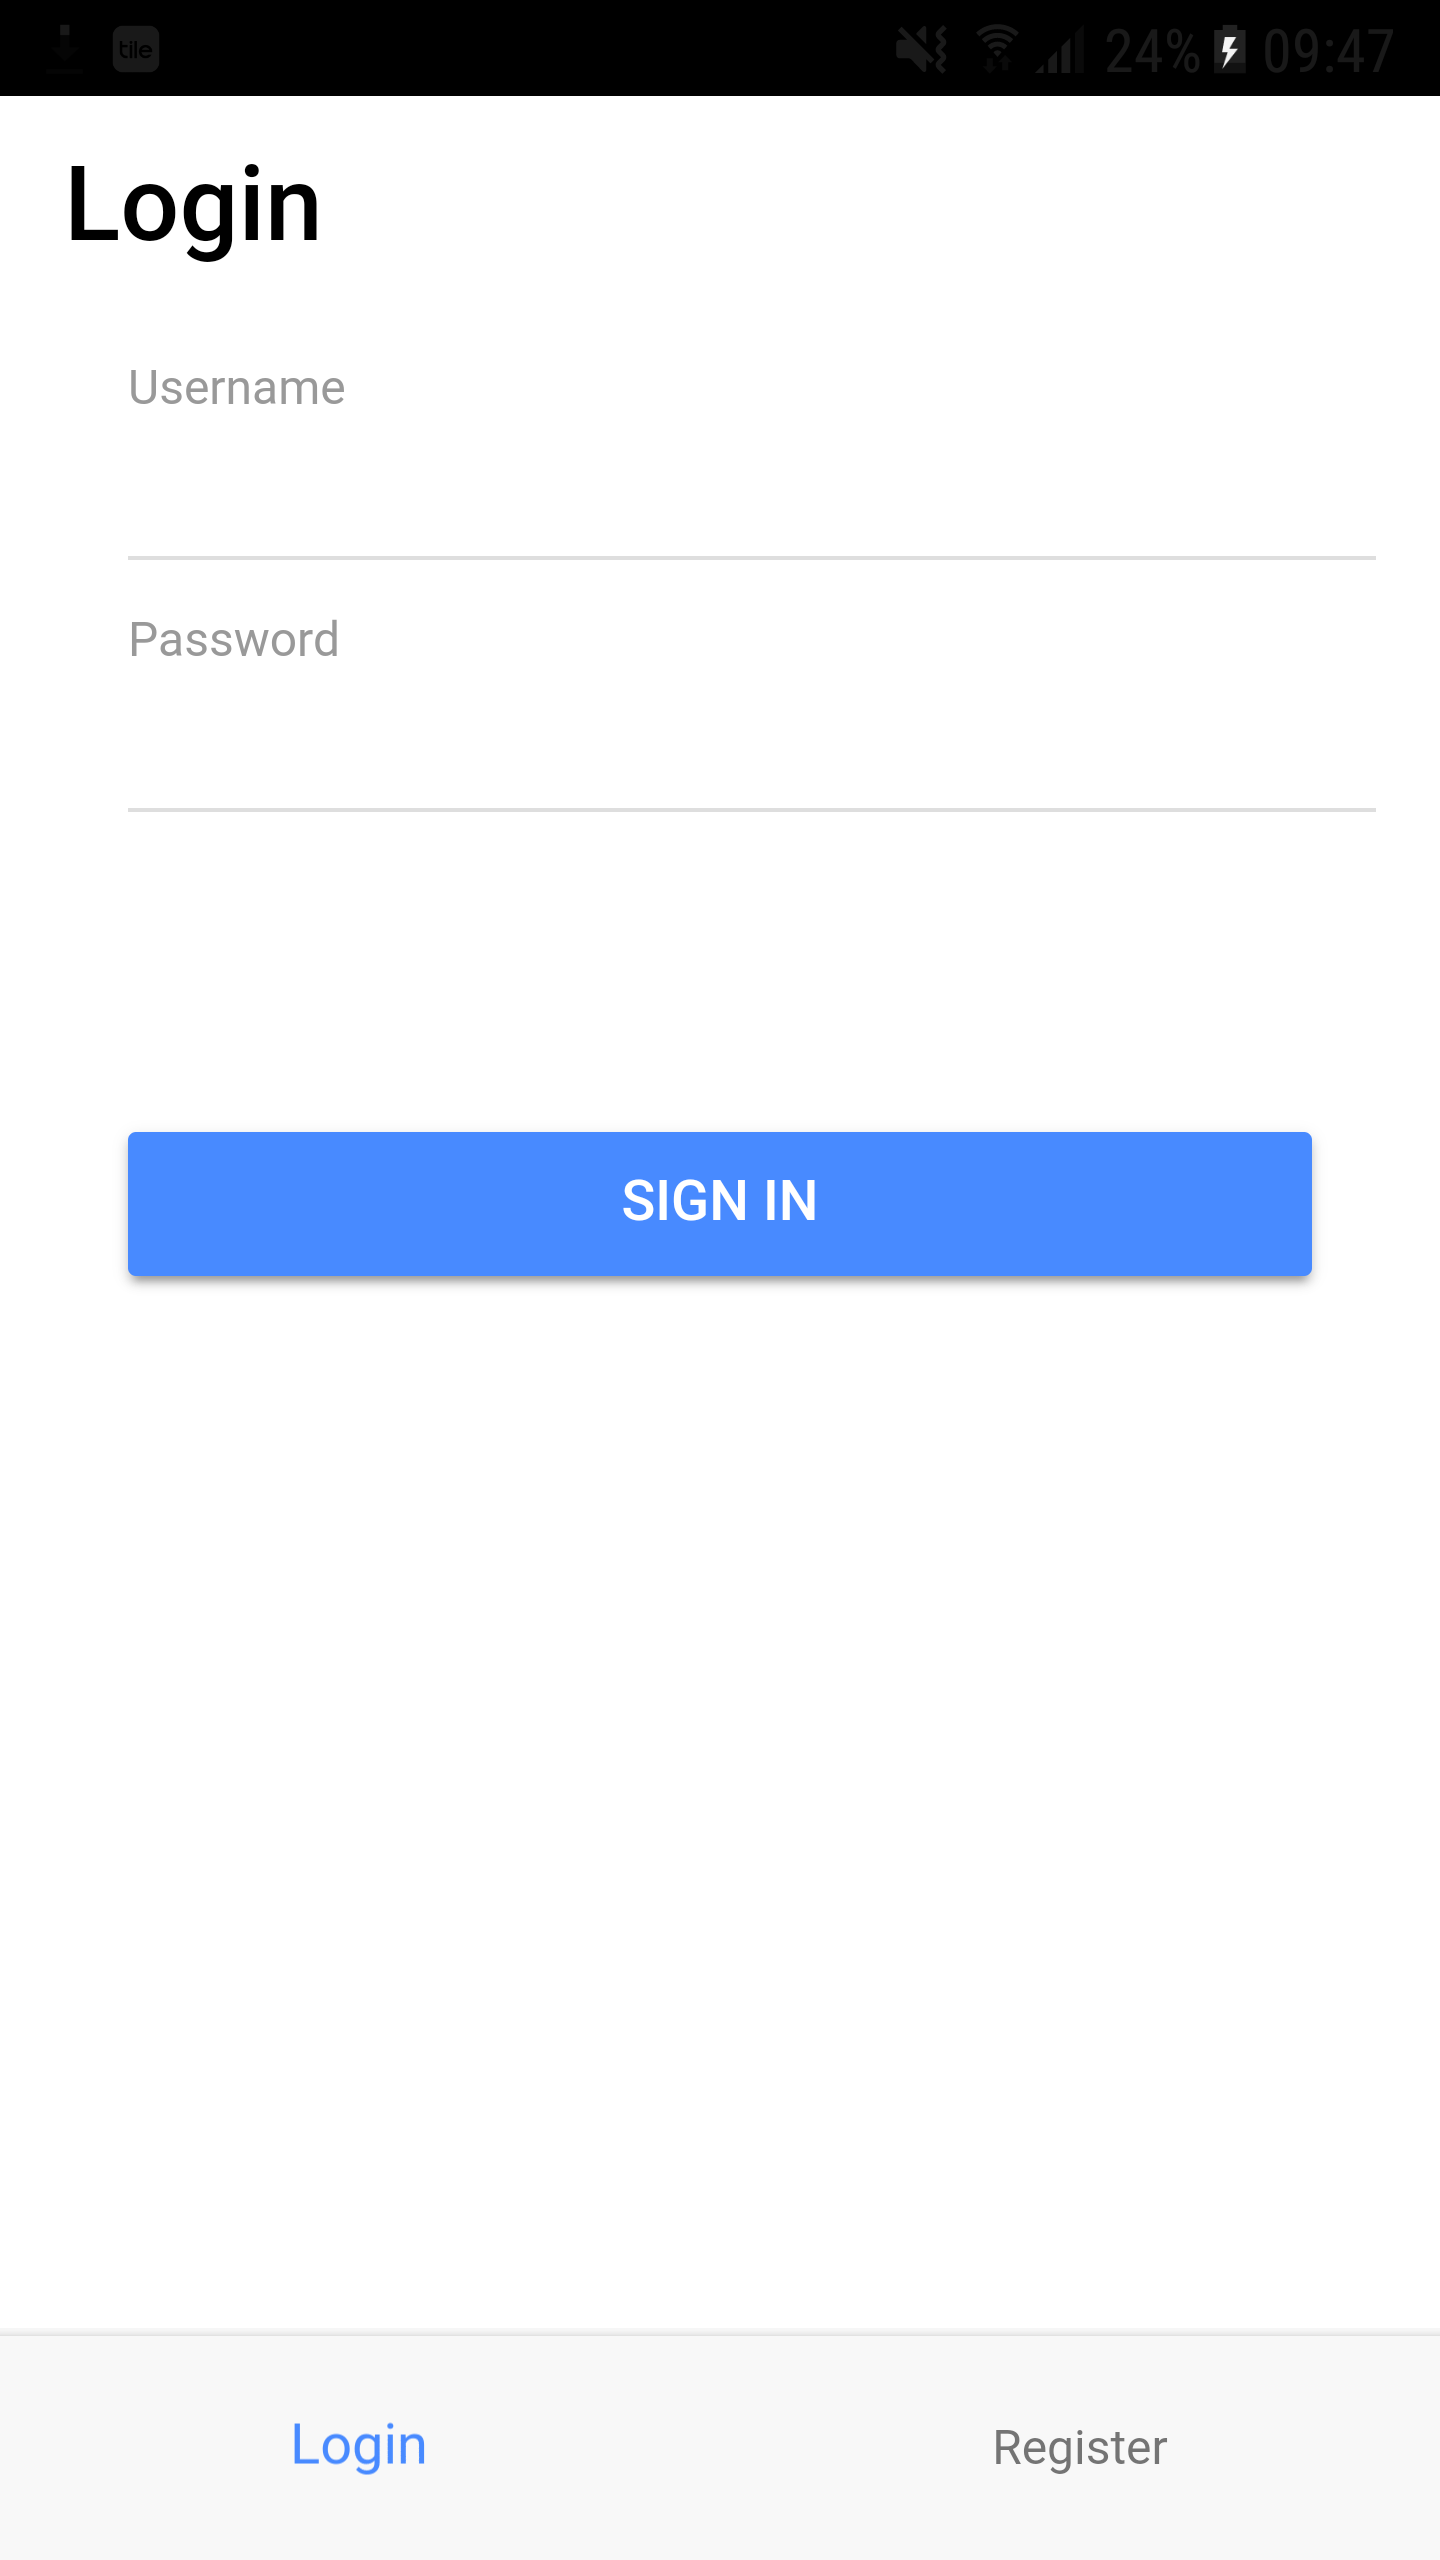
\includegraphics[width=0.4\textwidth]{images/login_page}}
	\quad
	\subfloat[Ekran rejestracji]{\label{odnosnik}
		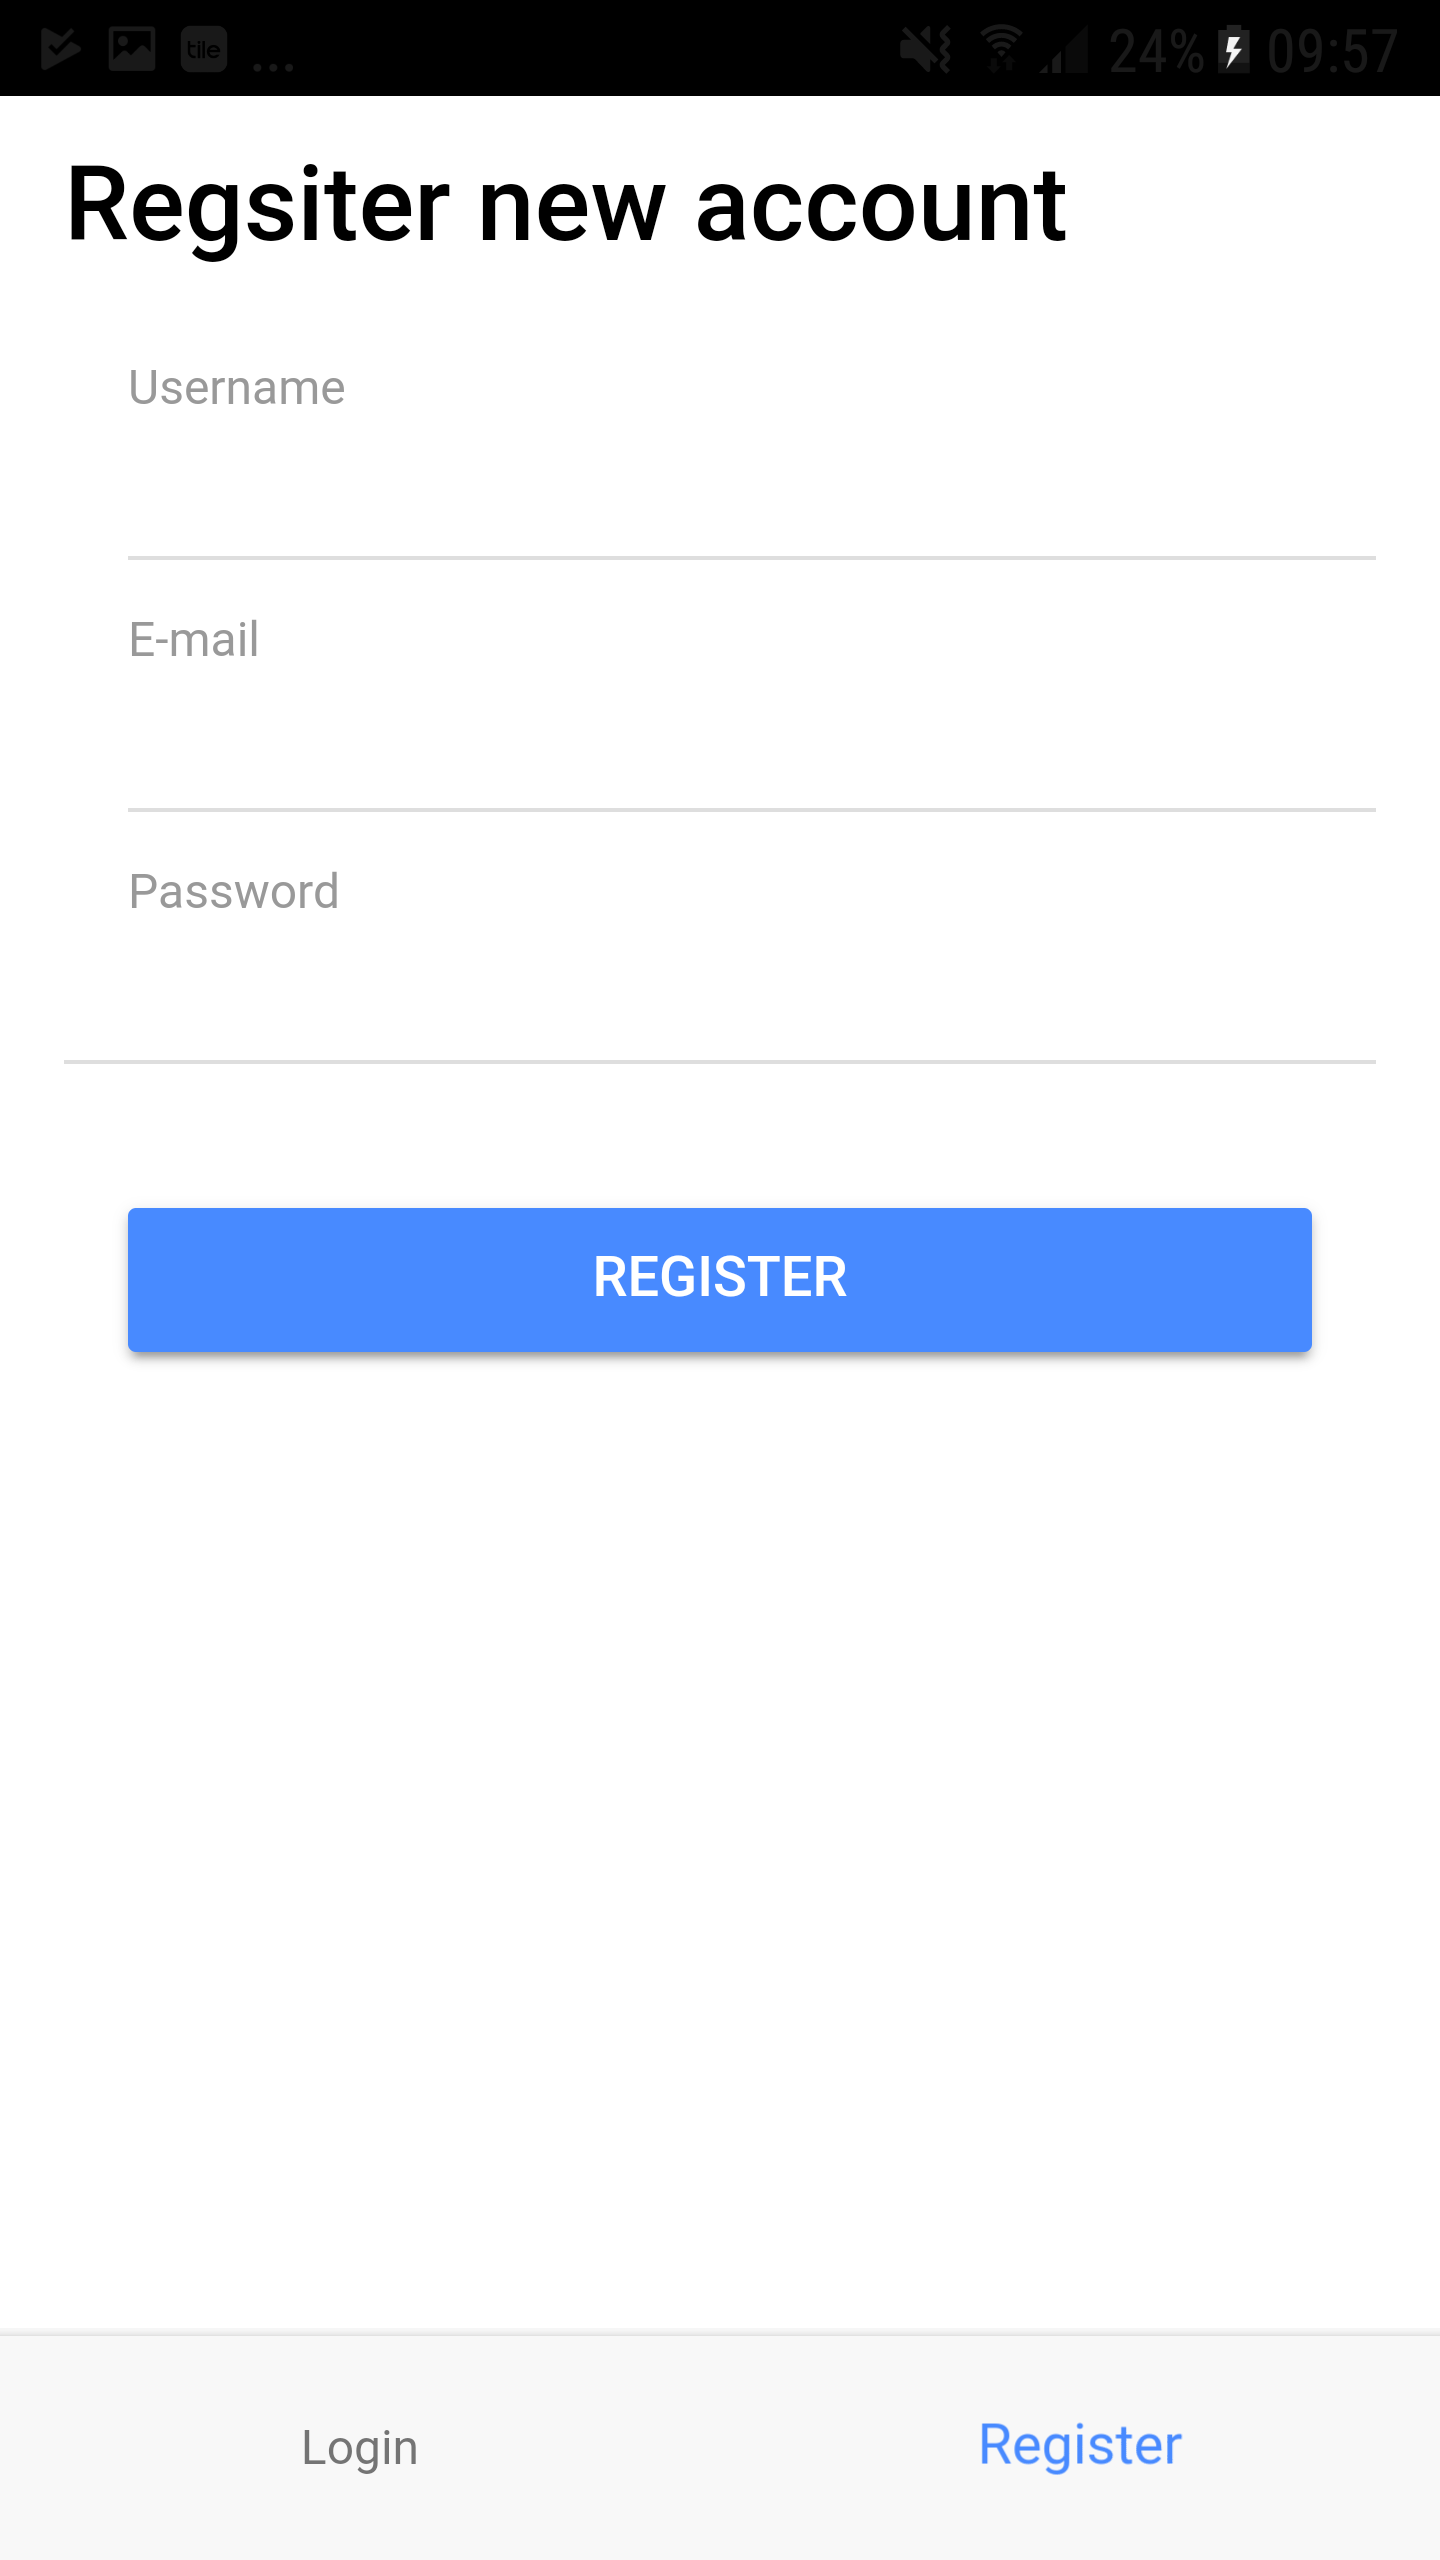
\includegraphics[width=0.4\textwidth]{images/register_page}}
	\caption{Ekrany logowania i rejestracji}
	\label{fig:registerpage}
\end{figure}

%\begin{wrapfigure}[15]{R}{0.4\textwidth}
%	\centering
%	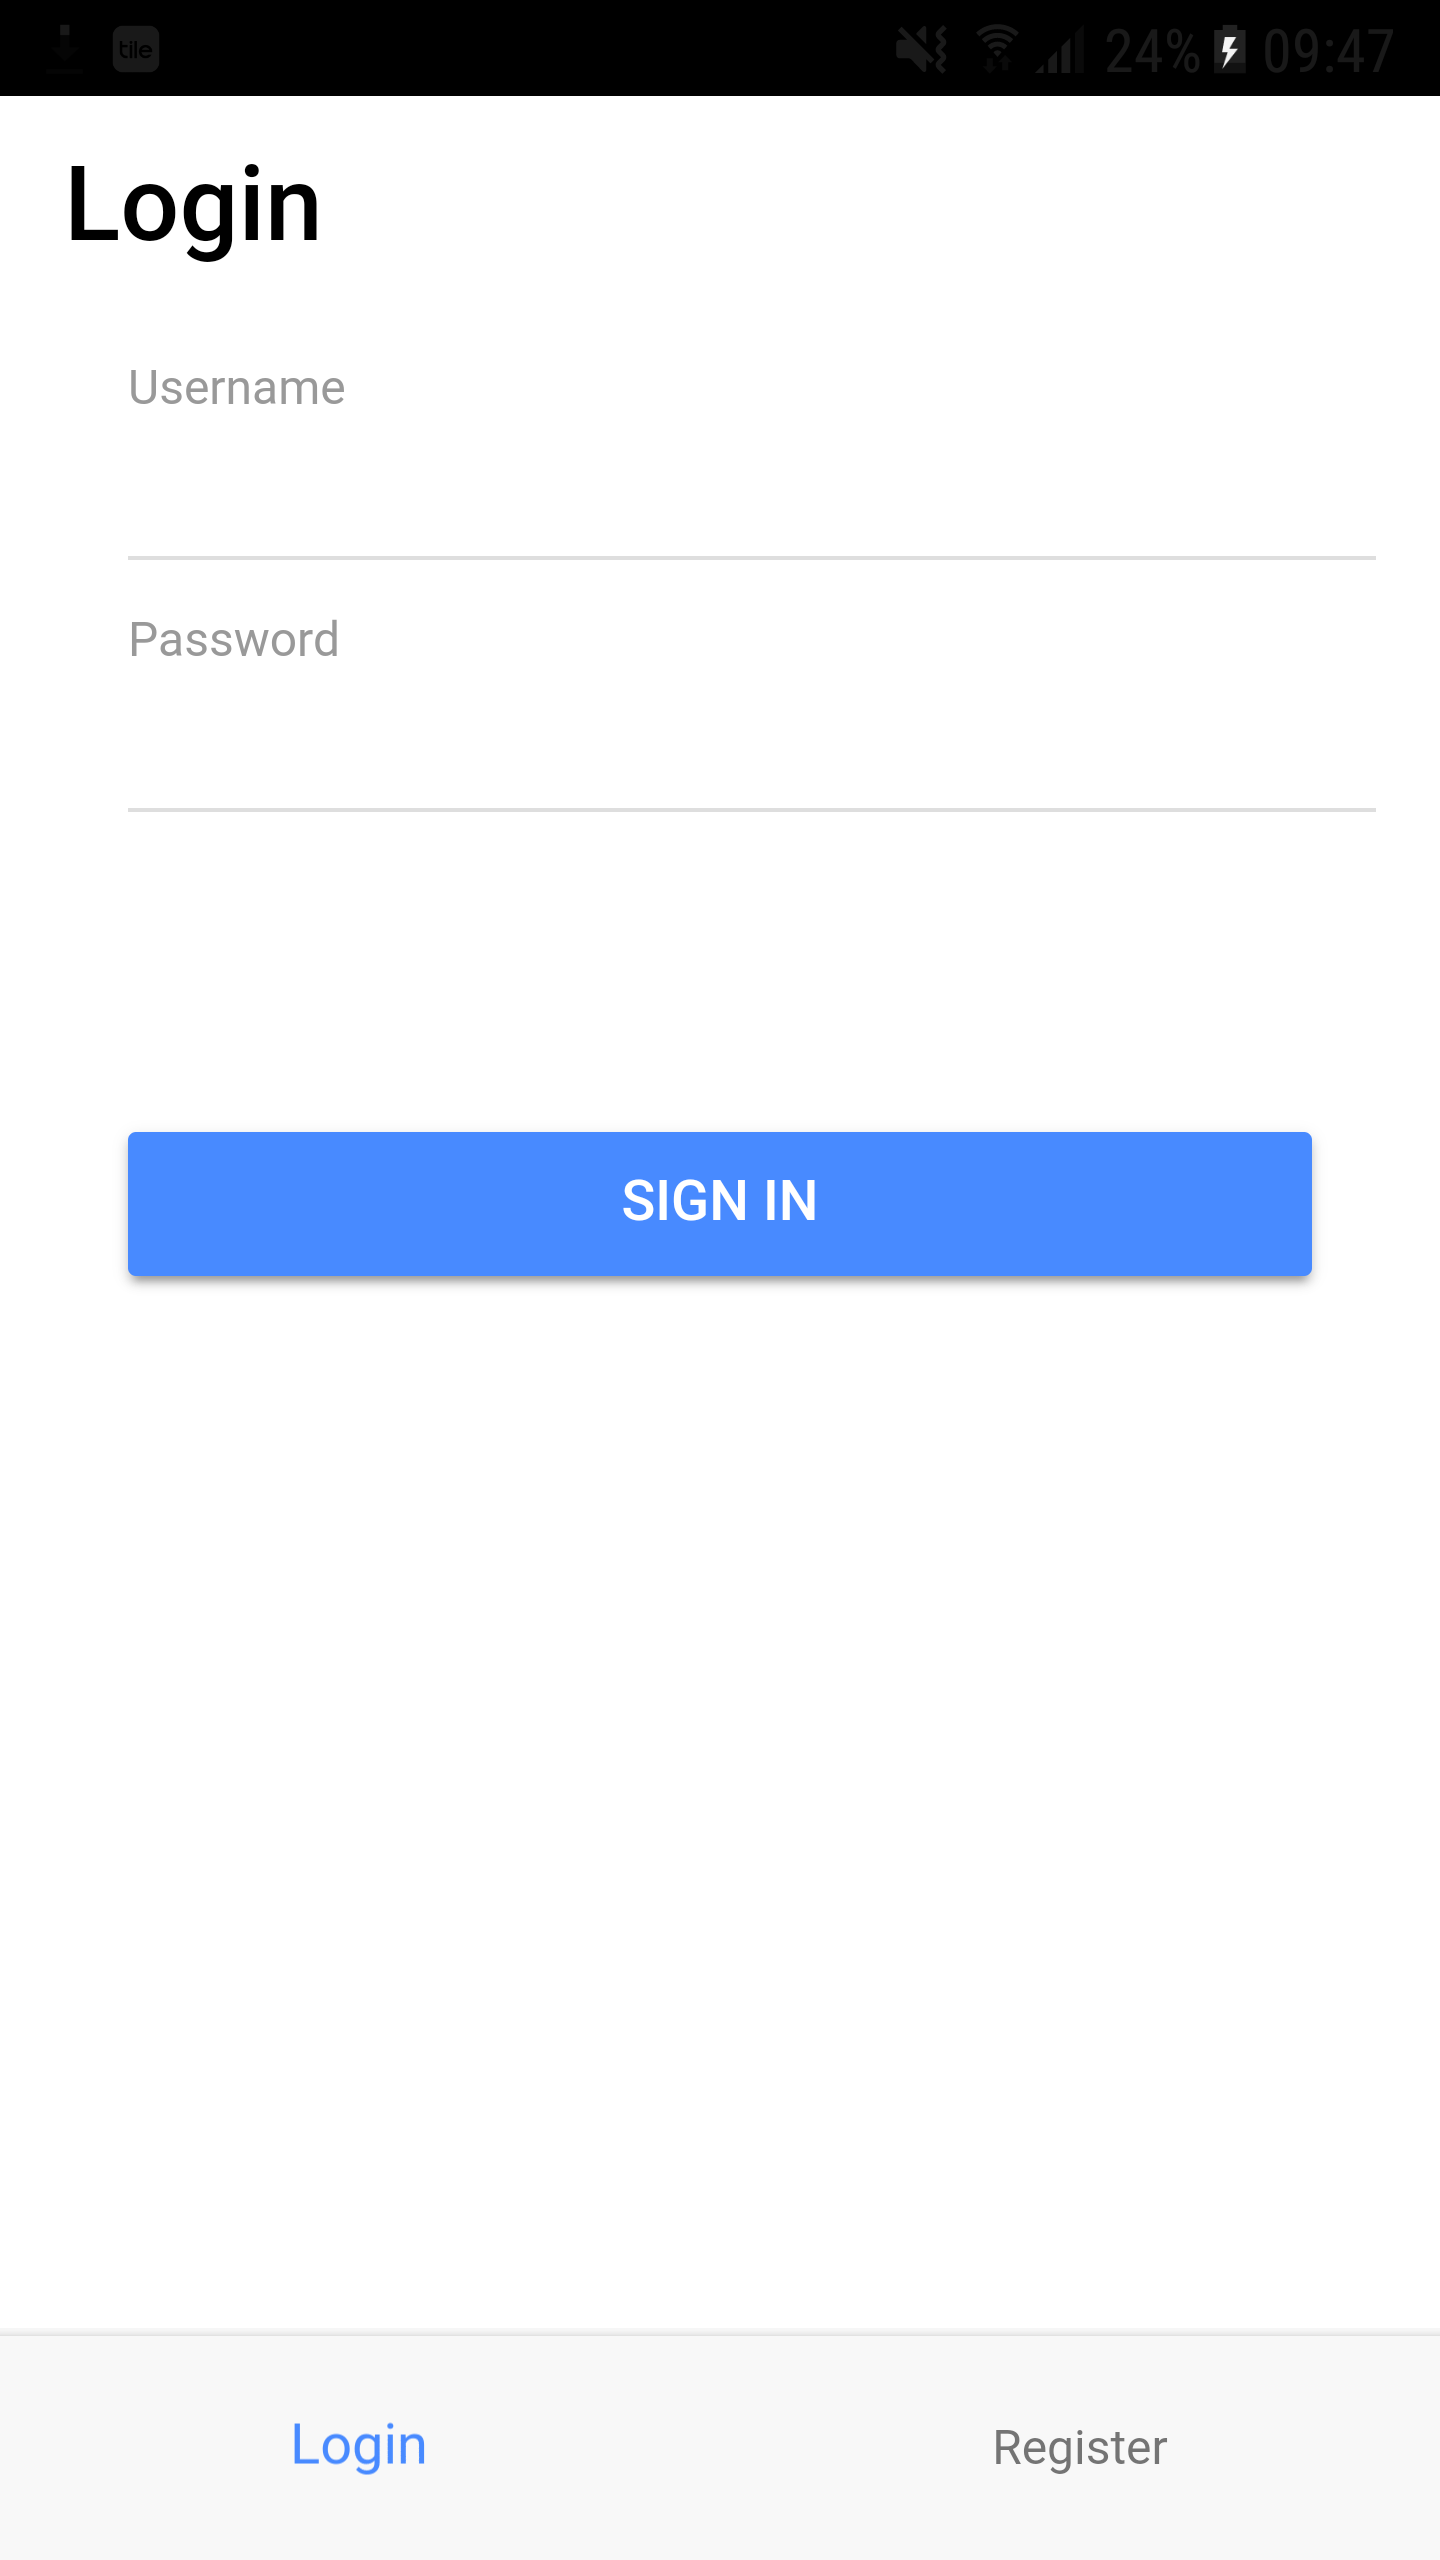
\includegraphics[width=0.4\textwidth]{images/login_page}
%	\caption{Ekran logowania.}
%\end{wrapfigure}

Użytkownik w celu korzystania z aplikacji musi być zalogowany. Pierwsze uruchomienie aplikacji skutkuje uruchomieniem ekranu logowania. W przypadku gdy użytkownik wcześniej zalogował się, a token dostępu nie wygasł, wówczas dostępny jest ekran główny aplikacji. Ze względu na asynchroniczną komunikację z serwerem poprzez zapytania HTTP, użytkownik w trakcie oczekiwania na odpowiedź ma przedstawiony ekran ładowania. W przypadku otrzymania błędu lub wykonania zabronionej operacji na serwerze, użytkownik otrzyma powiadomienie na dole ekranu.

%\begin{wrapfigure}[25]{R}{0.6\textwidth}
%	\centering
%	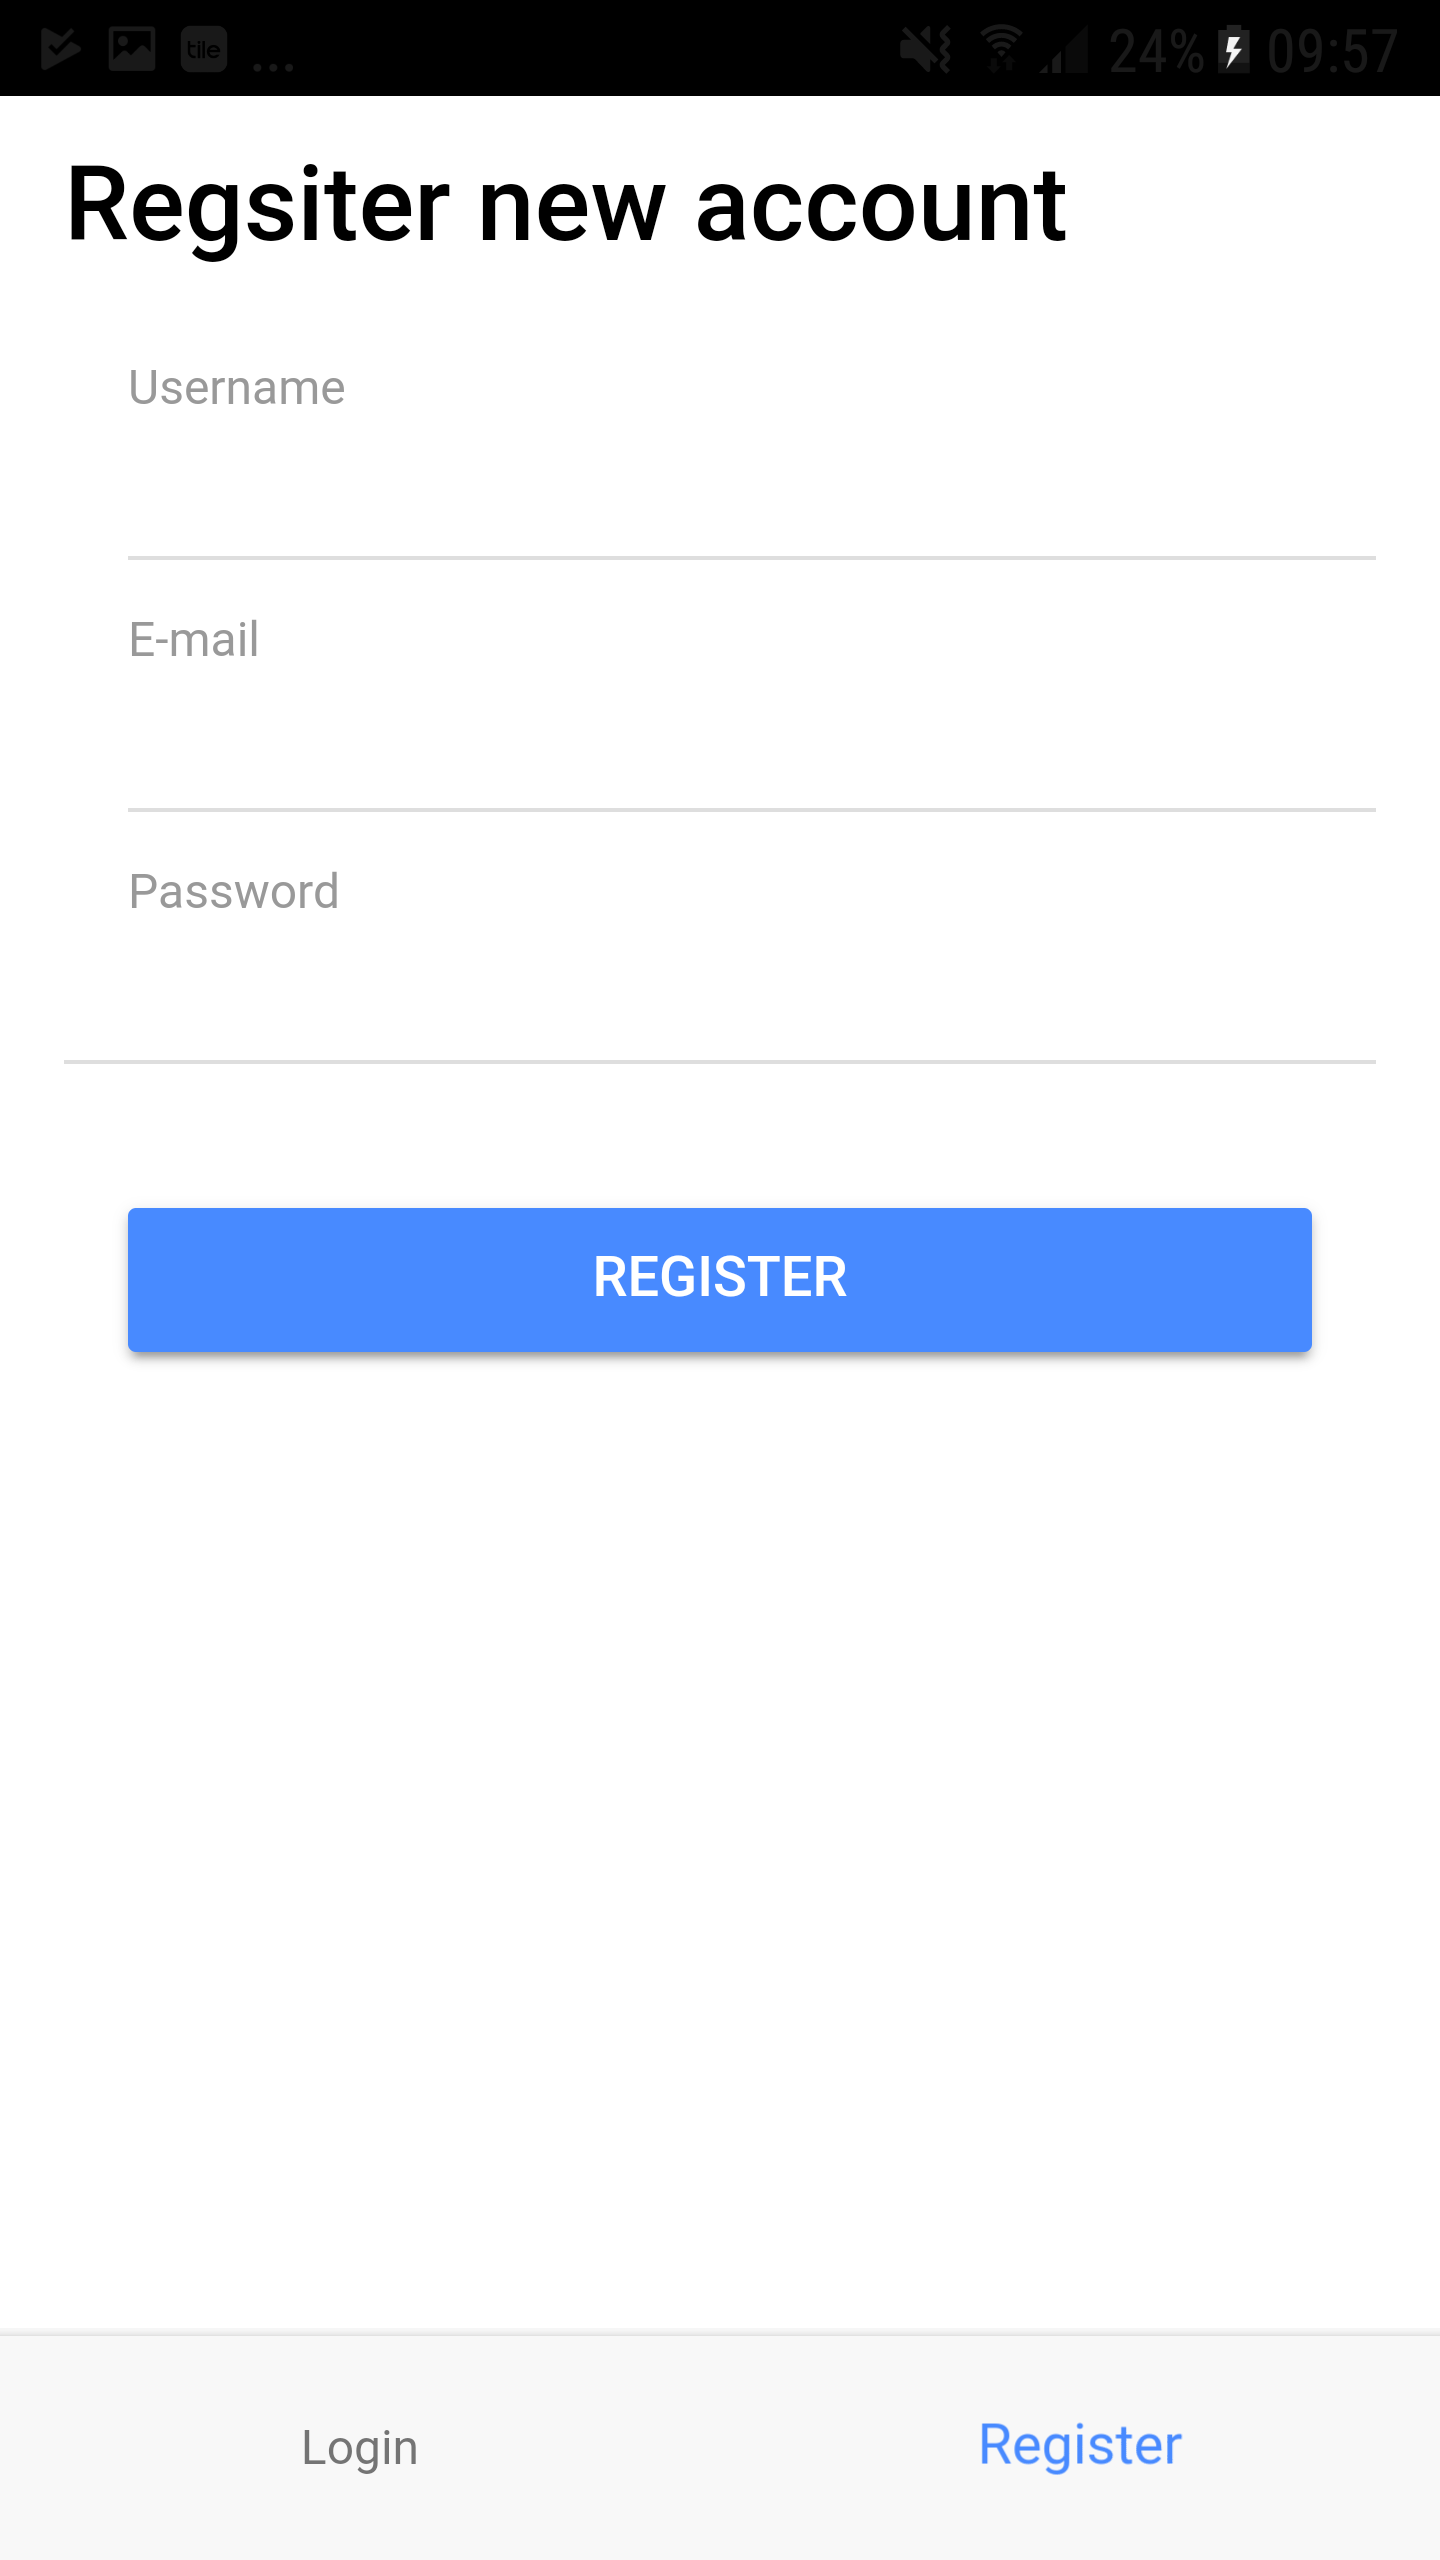
\includegraphics[width=0.8\linewidth]{images/register_page}
%	\caption{Ekran rejestracji.}
%	\label{fig:registerpage}
%\end{wrapfigure}

W przypadku gdy użytkownik nie posiada konta, zalecane jest skorzystanie z zakładki "Rejestracja". Umożliwia ona wpisanie podstawowych informacji niezbędnych do założenia konta. Zostały nałożone również restrykcje dotyczące polityki bezpieczeństwa konta. W związku z tym podczas rejestracji użytkownik jest proszony o:
\begin{itemize}[noitemsep]
	\item podanie adresu e-mail,
	\item podanie unikalnej nazwy użytkownika,
	\item ustawienie hasła zawierającego co najmniej trzy znaki.
\end{itemize} 
}
\newpage
\section{Zarządzanie zdjęciami}{

Pomyślna rejestracja oraz zalogowanie użytkownika przenoszą go do ekranu głównego aplikacji. Omawiany ekran znajduje się na rysunku \ref{mainView}. Pierwszy widok zawiera instrukcje zachęcające do zrobienia nowego zdjęcia lub wybrania go z galerii. Ponadto na ekranie dostępne są dodatkowe zakładki - "History" oraz "Contact". Użytkownik ma możliwość wylogowania się dzięki przyciskowi "Logout" znajdującemu się w prawym górnym rogu ekranu. Pierwszy ekran umożliwia przesłanie zdjęcia do serwera aplikacji w celu dalszego przetwarzania. Aby zrobić zdjęcie, należy wybrać przycisk "TAKE PHOTO", który uruchomi kamerę. Aplikacja będzie oczekiwała do momentu przekazania zdjęcia z urządzenia mobilnego. W przypadku wybrania przycisku "SELECT FROM GALLERY", aplikacja uruchomi systemowy eksplorator zdjęć. Wybór jednego z nich będzie równoznaczny dla aplikacji ze zrobieniem zdjęcia z aparatu. Aplikacja po wybraniu obrazu wyświetli go na ekranie głównym oraz udostępni przyciski "Send" oraz "Remove". Wybranie przycisku "Send" uruchomi udostępnienie zdjęcia na serwer. W przypadku przycisku "Remove" przesyłanie zostanie anulowane. Stan aplikacji został przedstawiony na rysunku \ref{uploadView}.

\begin{figure}[htb]
	\centering
	\label{beforeClasification}
	\noindent\begin{minipage}
		{0.4\textwidth}\raggedleft		\includegraphics[width=\linewidth,height=9cm]{"images/home_page"}
		\caption{Próbki obrazów poddane klasyfikacji produktów.}
		\label{mainView}
	\end{minipage}
	\begin{minipage}{0.4\textwidth}
		\includegraphics[width=\linewidth,height=9cm]{"images/upload_page"}
		\caption{Próbki obrazów poddane klasyfikacji produktów.}
		\label{uploadView}
	\end{minipage}
\end{figure}